\section{Аналитическая часть}

В данной части будет идти речь о корпусах текстов, видах текстов и текстовых разметок. % XXX будет идти или идет?

\subsection{Корпуса текстов}

Корпусная лингвистика --- раздел компьютерной лингвистики, занимающийся разработкой общих принципов построения и использования лингвистических корпусов (корпусов текстов) с применением компьютерных технологий.
Под лингвистическим, или языковым, корпусом текстов понимается большой, представленный в машиночитаемом формате, унифицированный, структурированный, размеченный, филологически компетентный массив языковых данных, предназначенный для решения конкретных лингвистических задач. \cite[с. 5]{cl}

\subsubsection{Виды}

В таблице \ref{tab:coc} ниже представлена классификация корпусов по некоторым признакам.

\begin{table}[H]
\centering
        \caption{Классификация корпусов \cite[с. 16]{cl}}
		\label{tab:coc}
        \begin{adjustbox}{width=\textwidth}
            \begin{tabular}{|p{0.3\textwidth}|p{0.7\textwidth}|}
        \hline
        Признак & Тип корпуса \\
        \hline
        \hline
        Цель & многоцелевые, специализированные \\
        \hline
        % Параллельность & одноязычные, двуязычные, многоязычные \\
        Параллельность & параллельные, сопоставимые (псевдопараллельные) \\
        \hline
        Тип языковых данных & письменные, устные (речевые), смешанные \\
        \hline
        <<Литературность>> & литературные, диалектные, разговорные, терминологические, смешанные \\
        \hline
        Жанр & литературные, фольклорные, драматургические, публицистические \\
        \hline
        Назначение & исследовательские, иллюстративные \\
        \hline
        % Динамичность & динамические, статические \\
        % \hline
        Разметка & размеченные, неразмеченные \\
        \hline
        Характер разметки & морфологические, синтаксические, семантические, анафорические и т. д. \\
        \hline
        % Доступность & свободно доступные, коммерческие, закрытые \\
        % \hline
        Объем текстов & полнотекстовые, <<фрагментнотекстовые>> \\
        \hline
		\end{tabular}
        \end{adjustbox}
\end{table}

\newpage

В данной работе особое внимание уделяется параллельным корпусам, так как именно для работы с таким видом корпусов будет разрабатываться база данных. % XXX meh, уделяется; будет разрабатываться

Параллельный корпус --- это двуязычный корпус.
В нем хранится два множества текстов --- оригиналов и их переводов.
Работа с корпусом (выравнивание, разметка, поиск) производится сразу с двумя текстами. %, ровно один из которых оригинальный.

Для возможности использования параллельного корпуса в качестве инструмента исследования, тексты должны быть выровнены --- отдельные фрагменты оригинала должны совпадать с соответствующими фрагментами перевода \cite{postnauka}.

Подробнее о применении, устройстве и проблематике параллельных корпусов будет говориться в следующих подразделах.

\subsubsection{Применение}

В данном подразделе рассматриваются некоторые применения параллельных корпусов.

\subsubsection*{Машинный перевод}

Машинный перевод (MT) представляет собой процесс перевода с одного естественного языка на другой с использованием компьютеров.
Параллельные корпусы используются, как правило, для систем статистического машинного перевода, принцип работы которого заключается в анализе больших массивов параллельных текстов и в выборе для перевода наиболее часто встречающихся вариантов.

% \subsubsection*{Обработка естественного языка (NLP)}

% \blindtext

\subsubsection*{Кросс-языковой поиск информации (CLIR)}

Параллельные корпуса могут использоваться для обучения моделей, способных искать информацию на одном языке и предоставлять информацию на другом.

\subsubsection*{Разработка словарей и учебных материалов}

Параллельные корпуса могут использоваться при разработке словарей и учебных материалов, например, для создания примеров употребления слов в контексте.

\subsubsection*{Лингвистические исследования}

В лингвистических исследованиях параллельные корпуса могут использоваться для подсчета частот встречаемости различных языковых элементов.
Статистическими методами на материале корпуса можно определить, какие слова регулярно встречаются вместе и, таким образом, могут быть отнесены к устойчивым словосочетаниям. \cite[с. 81]{cl}

\subsubsection{Устройство}

Параллельные корпуса устроены таким образом, чтобы решались поставленные перед ними задачи.
Типичная задача параллельных корпусов включает в себя поиск по корпусу по словам или по тегам.

Для осуществления поиска по корпусу, в нем должна храниться следующая информация:
\begin{itemize}
    \item тексты и их метаданные,
    \item выравнивание,
    \item теги и аннотации.
\end{itemize}

Теги и аннотации, наряду с выровненными текстами обычно \cite{cl, survey, ruscorpora, opencorpora} хранятся в формате XML.
Но хранение информации в таком формате имеет ряд недостатков:
\begin{itemize}
    \item Использование XML-тегов приводит к увеличению размера файлов и дублированию информации;
    \item Поиск по текстовым файлам зачастую медленнее поиска по бинарным, особенно при большом количестве хранимой информации;
    \item Ту же самую информацию можно хранить в виде бинарных файлов, используя при этом меньше места.
\end{itemize}

\subsection{Тексты}

% FIXME future -> present
В данном разделе будут рассмотрены виды текстовых разметок и структура технических текстов, а также будет описана проблема, возникающая при автоматическом выравнивании текстов на уровне терминов.

\subsubsection{Виды разметок}

В данном подразделе описаны некоторые виды текстовых разметок.

\subsubsection*{Морфологическая}

Представление в корпусе информации о морфологических формах и значениях (часть речи, род, падеж, вид...) является самостоятельной научной проблемой. \cite{ruscorpora}

В национальном корпусе русского языка \cite{ruscorpora} морфологическая информация, приписываемая произвольной словоформе в тексте, содержательно делится на четыре типа информации:
\begin{enumerate}
    \item Лексема (лемма), которой принадлежит словоформа (указывается «словарная запись» данной лексемы и ее принадлежность к той или иной части речи).
    \item Множество грамматических признаков данной лексемы, или словоклассифицирующие характеристики (например, род для существительного, переходность для глагола).
    \item Множество грамматических признаков данной словоформы, или словоизменительные характеристики (например, падеж для существительного, число для глагола).
    \item Информация о нестандартности грамматической формы, орфографических искажениях и т. п.
\end{enumerate}

Примеры тегов морфологической аннотации в НКРЯ \cite{ruscorpora}:
\begin{itemize}
    \item S	--- существительное (яблоня, лошадь, корпус, вечность);
    \item A	--- прилагательное (коричневый, таинственный, морской);
    \item NUM --- числительное (четыре, десять, много);
    \item m	--- мужской род (работник, стол);
    % \item f	--- женский род (работница, табуретка);
    \item anim --- одушевленность (человек, ангел, утопленник);
    % \item inan --- неодушевленность (рука, облако, культура);
    \item sg --- единственное число (яблоко, гордость);
    % \item pl --- множественное число (яблоки, ножницы, детишки);
    \item nom --- именительный падеж (голова, сын, степь, сани, который);
    % \item gen --- родительный падеж (головы, сына, степи, саней, которого);
    % \item dat --- дательный падеж (голове, сыну, степи, саням, которому);
    \item persn	--- личное имя (Иван, Дарья, Леопольд, Эстер, Гомер, Маугли).
\end{itemize}

\subsubsection*{Синтаксическая}

Синтаксическую структуру предложения можно представить в виде дерева зависимостей, в котором каждая дуга (стрелка) идет из главного слова (<<хозяина>>) в зависимое слово (<<слугу>>) и помечена именем определенного синтаксического отношения.
Каждое слово предложения, кроме одного (называемого вершиной предложения), зависит только от одного хозяина и только по одному из синтаксических отношений.
Отношения связывают отдельные слова, а не словосочетания (за исключением специальных случаев).
В синтаксических группах (например, в сочиненной именной группе или придаточной клаузе) один из членов группы выступает в качестве представителя группы во внешних связях, объявляется вершиной группы, а остальные члены группы синтаксически зависят от него. \cite{ruscorpora}

На рисунке ниже представлена синтаксическая разметка в двух форматах --- в формате универсальных зависимостей (UD) и в формате СинТагРус.

\begin{figure}[H]
	\centering
	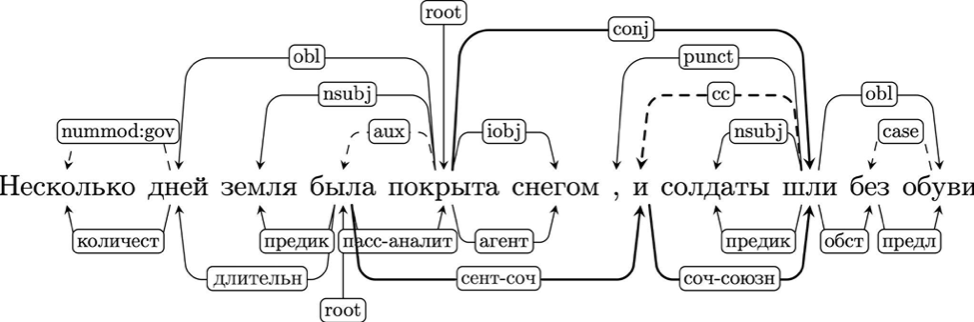
\includegraphics[width=0.9\textwidth]{img/syntax.png}
	\caption{Разметка предложения в формате UD (сверху) и СинТагРус (снизу). Стрелки отношений в сочиненной группе выделены. Функциональные отношения UD обозначены пунктирными стрелками.}
	\label{fig:syn}
\end{figure}

\subsubsection*{Семантическая}

При семантической разметке большинству слов в тексте приписывается один или несколько семантических и словообразовательных признаков, например, 'лицо', 'вещество', 'пространство', 'скорость', 'движение', 'обладание', 'свойство человека', 'диминутив', 'отглагольное имя' и т. п.
В национальном корпусе русского языка \cite{ruscorpora} используется фасетная классификация, при которой одно слово может попадать в несколько классов.

\subsubsection*{Метаразметка}

Под метаразметкой понимается приписывание тексту атрибутов, характеризующих обстоятельства его создания, автора, тематику, жанровые особенности и др. \cite{ruscorpora}

\subsubsection{Технические тексты и их структура}

Когда кто-то называет текст <<техническим>> в повседневной жизни, под этим обычно понимается сложность его восприятия.
% FIXME too long
В ученых кругах --- наоборот, <<техничность>> текста означает б\textbf{о}льшую доступность его обработки вследствие лишенности фигуративного языка, минимального использования переносных значений слов и возможности понимать его содержимое в буквальном смысле. \cite{tt}

Но четкого и общепринятого определения у понятия <<технический текст>> нет.

Тем не менее, у людей есть общее представление о том, какой текст является техническим, а какой --- нет.

% FIXME too long
Исходя из предположения о том, что среднестатистический человек способен оценивать <<техничность>> текста, исследование \cite{tt}, включало проведение массового опроса участников, в результате которого были выделены критерии, значения которых обычно выше у технических текстов.

У технических текстов преобладают следующие критерии:
\begin{itemize}
    \item наличие заголовков,
    \item определение темы и фокусировка на ней,
    \item предоставление знаний,
    \item серьезность и объективность,
    \item логичность и последовательность,
    \item иерархическая организация,
    \item использование специализированной терминологии.
\end{itemize}

Проанализировав ряд текстов на предмет их соответствия указанным выше критериям, становится возможным выявить структуру, характерную техническим текстам, а именно:
\begin{enumerate}
    \item Резюме, аннотация --- краткое описание содержания текста.
    \item Введение --- знакомство с проблемой.
    \item Теоретическая часть --- более глубокое знакомство с проблемой, знакомство читателя с методологией исследования и обоснованный выбор методов, которые будут использоваться в ходе исследования.
    \item Методология --- описание применения выбранных методов в ходе исследования.
    \item Результаты --- представление полученных результатов.
    \item Обсуждение и анализ результатов.
    \item Заключение.
\end{enumerate}

\subsubsection{Проблема терминов}

Выравнивание текстов на уровне секций, абзацев и предложений обычно не представляет трудности, и часто такое выравнивание можно автоматизировать.
Проблемы возникают при попытке выровнять тексты на уровне терминов.
Автоматически такое выравнивание произвести бывает сложно.
Причина сложности автоматического выравнивания на уровне терминов будет рассмотрена ниже на примере фразеологизмов.

Набор слов в фразеологизмах может иметь разные значения в зависимости от контекста.
Например, предложение <<It was a piece of cake>> нельзя перевести однозначно, не зная контекста, в котором оно употреблено.

В контексте 
\begin{itemize}
    \item Was it difficult?
    \item It was a piece of cake.
\end{itemize}
его можно перевести, как <<было просто>>, а в контексте
\begin{itemize}
    \item What was in the box?
    \item It was a piece of cake.
\end{itemize}
оно точно имеет отношение к куску пирога.

Таким образом, для корректности перевода, машинный перевод должен учитывать контекст, в котором термин употреблен.
Но это и есть одна из задач, для решения которой параллельные корпуса и создаются изначально.
В этом и заключается проблема терминов.

% \subsection{Существующие параллельные корпуса}

% TODO: Надо ли описывать 3-4 существующих параллельных корпуса, делать сравнительную таблицу по критериям:
% - Способ хранения текстов и разметки
% - Возможность загрузки собственных текстов
% - Возможность разметки собственных текстов
% и подводить к актуальности разработки БД?

\subsection{Вывод}

В данной части была рассмотрена предметная область параллельных корпусов текстов, были описаны виды текстовых разметок, структура технический текстов и проблема, возникающая при попытке автоматизации выравнивания текстов на уровне терминов.
